\subsection{Fresh-agent attempts (\texttt{\FRESHRUN}), the lead result}
\label{sec:results-fresh}
% Every number is a macro of generated/fresh/numbers.tex (\fv{key}); evidence_ledger_fresh.md names its file and field.
% Sources: results/runs/fresh-v1/{manifest,analysis,analysis_sensitivity}.json; docs/decision_log.md D61, D62.
Run \texttt{\FRESHRUN} graded the eight verifiers of each family (C1--C4, B1, B2 and the two label-support verifiers) on \fv{run.candidates} candidates under harness \fv{run.harness}, every pair \fv{run.repeats} times, with no unresolved outcome (\fv{run.pairs} pairs; \fv{run.unresolved} unresolved). Of the \fv{attempts} attempts, \fv{attempts.excluded} is excluded by the reviewed audit (\texttt{\fv{excluded.1}}); each distinct graded patch then counts once, leaving \fv{units} units, \fv{units.invalid} invalid and \fv{units.valid} valid under D19. \textbf{Every rate in this subsection rests on model-proposed labels}; no human label exists. With four families the exact sign-flip test cannot give a two-sided $p$ below \fv{cmp.floor.two}, so the subsection is descriptive. The per-family display is primary (Table~\ref{tab:fresh-family}, Figure~\ref{fig:fresh-fa}).

\IfFileExists{generated/fresh/fresh_per_family.tex}{\begin{table}[t]\centering\footnotesize\setlength{\tabcolsep}{4pt}
\caption{Per-family false acceptance and false rejection on the fresh-agent stratum, the primary display (protocol \S15.7), under rule D19's labels: 29 invalid and 50 valid attempts, each distinct graded patch once (79 graded patches; excluded by the reviewed audit: \texttt{CS-02-fresh-A-final-1}). Run \texttt{fresh-v1} graded every pair 3 times under harness 0.3.5 (672 pairs, 0 unresolved). n/a: the family has no attempt of that kind. The second labeler's view: Table~\ref{tab:fresh-family-labeler}. $^{\diamond}$Automated pilot; model-proposed labels, no human labels; 4 controlled families; descriptive (\S\ref{sec:intro}).}\label{tab:fresh-family}
\begin{tabular}{lrrrrrrrrrr}\toprule  & \multicolumn{5}{c}{False acceptance (accepted/invalid)} & \multicolumn{5}{c}{False rejection (rejected/valid)} \\\cmidrule(lr){2-6}\cmidrule(lr){7-11} Condition & CS-01 & CS-02 & CS-03 & CS-04 & Pooled & CS-01 & CS-02 & CS-03 & CS-04 & Pooled \\\midrule
C1 initial-only, plain & 10/10 & 0/2 & 4/7 & 10/10 & 24/29 & 10/10 & 0/17 & 3/13 & 0/10 & 13/50 \\
C2 initial-only, audited & 10/10 & 0/2 & 4/7 & 10/10 & 24/29 & 10/10 & 0/17 & 3/13 & 0/10 & 13/50 \\
C3 correction-aware, plain & 0/10 & 2/2 & 0/7 & 0/10 & 2/29 & 0/10 & 0/17 & 0/13 & 0/10 & 0/50 \\
C4 correction-aware, audited & 0/10 & 2/2 & 0/7 & 0/10 & 2/29 & 0/10 & 0/17 & 6/13 & 0/10 & 6/50 \\
B2 session-LLM baseline & 0/10 & 2/2 & 0/7 & 0/10 & 2/29 & 0/10 & 0/17 & 2/13 & 0/10 & 2/50 \\
B1 repository tests & 0/10 & 0/2 & 0/7 & 0/10 & 0/29 & 8/10 & 17/17 & 9/13 & 0/10 & 34/50 \\
\bottomrule\end{tabular}\end{table}
}{\unfilled{fresh per-family table}}
\IfFileExists{generated/figures/fresh_fa_by_family.tex}{% Generated by `python paper/make_figures.py`; do not edit. Every value: paper/evidence_ledger_figures.md.
\begin{figure}[t]\centering
\ifdefined\includegraphics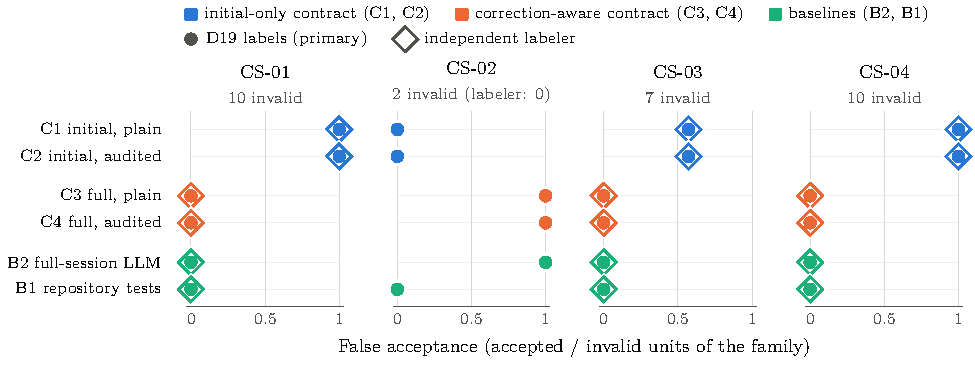
\includegraphics[width=\linewidth]{generated/figures/fresh_fa_by_family.pdf}%
\else\unfilled{figure fresh\_fa\_by\_family: main.tex must load graphicx}\fi
\caption{False acceptance per family on the fresh-agent stratum (run \texttt{fresh-v1}, an automated study), the per-family display of protocol \S15.7: for each condition, the share of a family's invalid units that it accepts, under D19 (filled circles) and under the independent labeler, a second labeling (open diamonds; a circle inside a diamond: both labelings give the same value). Each distinct graded patch counts once (79 units); under each family: its invalid units under D19, and under the labeler where that differs. \textbf{All labels are model proposals; no human labels exist.} Four controlled families: descriptive, not inferential. In CS-02 the 2 invalid units under D19 violate only the regression norm; the labeler, which has no regression part, labels both valid, so CS-02 has no labeler mark. C1 and C2 do not pass CS-01's reference solution. Colour: the contract source; counts: Table~\ref{tab:fresh-family}.}\label{fig:fresh-fa}
\end{figure}
}{\unfilled{fresh figure}}

\paragraph{Initial-only verifiers accept what the correction ruled out.} Of the \fv{cv.attempts} attempts that saw only the first request (\texttt{u1}), \fv{cv.n} violate a requirement the correction introduced (\fv{cv}; Table~\ref{tab:fresh-cv}). The verifiers generated from the initial request accept \fv{cv.c1.accepted} of these \fv{cv.n} (C1 and C2 alike). The correction-aware verifiers accept none (C3 \fv{cv.c3}, C4 \fv{cv.c4}), and neither do the full-session LLM baseline (B2 \fv{cv.b2}) and the repository tests (B1 \fv{cv.b1}). Pooled over the families, C1 accepts \fv{c1.fa} invalid units and rejects \fv{c1.fr} valid ones, against \fv{c3.fa} and \fv{c3.fr} for C3. The contrast is concentrated: C1's false acceptances come from three of the four families (\fv{c1.famfa}), and in CS-01 C1 also fails its own reference solution, so it rejects every valid unit there (C1 and C2 pass \fv{ref.c1} references, every other condition \fv{ref.c3}). The false acceptances that C3, C4 and B2 share (\fv{c3.fa} each) are CS-02's two units whose only violation is the regression norm (\S\ref{sec:analysis}).

\IfFileExists{generated/fresh/fresh_correction_violating.tex}{\begin{table}[t]\centering\footnotesize
\caption{\texttt{u1} attempts (given the first user request only) that violate a requirement the reference contract introduces after it, by family, and how many of them each condition accepts (accepted/violating), run \texttt{fresh-v1}, rule D19's labels. Last column: the invalid attempts whose only violated requirement is the regression norm (accepted/total); they violate no correction requirement. $^{\diamond}$Automated pilot; model-proposed labels, no human labels; 4 controlled families; descriptive (\S\ref{sec:intro}).}\label{tab:fresh-cv}
\begin{tabular}{lrrrrrr}\toprule  & CS-01 & CS-02 & CS-03 & CS-04 & Pooled & Regression only \\\midrule
Correction-violating \texttt{u1} attempts & 10/10 & 0/10 & 7/10 & 10/10 & 27/40 & 2 \\\midrule
C1 initial-only, plain & 10/10 & -- & 4/7 & 10/10 & 24/27 & 0/2 \\
C2 initial-only, audited & 10/10 & -- & 4/7 & 10/10 & 24/27 & 0/2 \\
C3 correction-aware, plain & 0/10 & -- & 0/7 & 0/10 & 0/27 & 2/2 \\
C4 correction-aware, audited & 0/10 & -- & 0/7 & 0/10 & 0/27 & 2/2 \\
B2 session-LLM baseline & 0/10 & -- & 0/7 & 0/10 & 0/27 & 2/2 \\
B1 repository tests & 0/10 & -- & 0/7 & 0/10 & 0/27 & 0/2 \\
\bottomrule\end{tabular}\end{table}
}{}

\paragraph{The comparisons that test the proposed machinery are null or negative.} None of the \fv{cmp.count} pre-specified paired comparisons reaches the floor of its test (Table~\ref{tab:fresh-comparisons}; the smallest two-sided $p$ is \fv{cmp.min.p.two}). The largest difference, C1 against C3 on false acceptance (\fv{cmp.c1-c3.fa.diff}, one-sided $p=\fv{cmp.c1-c3.fa.p.greater}$), is at its floor because only four families carry it. The audit (audit:v1) removed no false acceptance: C2 equals C1 on every unit, and C4 equals C3 on false acceptance but rejects \fv{c4.fr} valid units against C3's \fv{c3.fr}, all of them in CS-03, where the revision over-restricts inputs that the contract leaves open (\S\ref{sec:analysis}). The full-session LLM baseline B2 matches C3 and C4 on false acceptance (\fv{b2.fa}) and rejects \fv{b2.fr} valid units. On these four families, then, the information a correction carries matters, while the audit and the requirement contracts add nothing measurable on false acceptance beyond a test generator that sees the whole session.

\IfFileExists{generated/fresh/fresh_comparisons.tex}{\begin{table}[t]\centering\scriptsize\setlength{\tabcolsep}{4pt}
\caption{The 14 pre-specified paired comparisons on the same units, run \texttt{fresh-v1}, D19 labels. \textbf{All labels are model proposals; no human labels exist.} Metric (n): FA over the invalid or FR over the valid units. A$-$B: pooled difference; then the per-family differences. Disc.: A accepts \& B rejects / A rejects \& B accepts. $p$: exact sign-flip randomization p-values over the 4 families, on the pooled statistic ($>$: A$>$B, $<$: A$<$B, both one-sided; 2-s.: two-sided) and, last but one, two-sided on the family-mean statistic. With 4 families no one-sided $p$ below 0.0625 and no two-sided $p$ below 0.125 can occur; Floor: the smallest one-sided $p$ attainable given the families whose difference is zero. The smallest two-sided $p$ here is 0.25. Short names: C1--C4 contracts (initial or full, plain or audited), B2 full-session LLM, B1 repository tests. Four controlled families: descriptive, not inferential.}\label{tab:fresh-comparisons}
\begin{tabular}{lllrrrrrrrrrrr}\toprule A & B & Metric (n) & A$-$B & CS-01 & CS-02 & CS-03 & CS-04 & Disc. & $p_{>}$ & $p_{<}$ & $p$ 2-s. & $p$ 2-s.\ (mean) & Floor \\\midrule
C1 & C3 & FA (29) & \ensuremath{+}0.76 & \ensuremath{+}1.00 & \ensuremath{-}1.00 & \ensuremath{+}0.57 & \ensuremath{+}1.00 & 24/2 & 0.125 & 0.9375 & 0.25 & 0.625 & 0.0625 \\
C1 & C3 & FR (50) & \ensuremath{+}0.26 & \ensuremath{+}1.00 & 0.00 & \ensuremath{+}0.23 & 0.00 & 0/13 & 0.25 & 1 & 0.5 & 0.5 & 0.25 \\
C2 & C4 & FA (29) & \ensuremath{+}0.76 & \ensuremath{+}1.00 & \ensuremath{-}1.00 & \ensuremath{+}0.57 & \ensuremath{+}1.00 & 24/2 & 0.125 & 0.9375 & 0.25 & 0.625 & 0.0625 \\
C2 & C4 & FR (50) & \ensuremath{+}0.14 & \ensuremath{+}1.00 & 0.00 & \ensuremath{-}0.23 & 0.00 & 5/12 & 0.5 & 0.75 & 1 & 1 & 0.25 \\
C1 & C2 & FA (29) & 0.00 & 0.00 & 0.00 & 0.00 & 0.00 & 0/0 & 1 & 1 & 1 & 1 & 1 \\
C1 & C2 & FR (50) & 0.00 & 0.00 & 0.00 & 0.00 & 0.00 & 0/0 & 1 & 1 & 1 & 1 & 1 \\
C3 & C4 & FA (29) & 0.00 & 0.00 & 0.00 & 0.00 & 0.00 & 0/0 & 1 & 1 & 1 & 1 & 1 \\
C3 & C4 & FR (50) & \ensuremath{-}0.12 & 0.00 & 0.00 & \ensuremath{-}0.46 & 0.00 & 6/0 & 1 & 0.5 & 1 & 1 & 0.5 \\
B2 & C4 & FA (29) & 0.00 & 0.00 & 0.00 & 0.00 & 0.00 & 0/0 & 1 & 1 & 1 & 1 & 1 \\
B2 & C4 & FR (50) & \ensuremath{-}0.08 & 0.00 & 0.00 & \ensuremath{-}0.31 & 0.00 & 4/0 & 1 & 0.5 & 1 & 1 & 0.5 \\
B2 & C3 & FA (29) & 0.00 & 0.00 & 0.00 & 0.00 & 0.00 & 0/0 & 1 & 1 & 1 & 1 & 1 \\
B2 & C3 & FR (50) & \ensuremath{+}0.04 & 0.00 & 0.00 & \ensuremath{+}0.15 & 0.00 & 0/2 & 0.5 & 1 & 1 & 1 & 0.5 \\
B1 & C4 & FA (29) & \ensuremath{-}0.07 & 0.00 & \ensuremath{-}1.00 & 0.00 & 0.00 & 0/2 & 1 & 0.5 & 1 & 1 & 0.5 \\
B1 & C4 & FR (50) & \ensuremath{+}0.56 & \ensuremath{+}0.80 & \ensuremath{+}1.00 & \ensuremath{+}0.23 & 0.00 & 0/28 & 0.125 & 1 & 0.25 & 0.25 & 0.125 \\
\bottomrule\end{tabular}\end{table}
}{}

\paragraph{Repository tests reject valid work through tests the session agent added.} B1 accepts no invalid unit (\fv{b1.fa}) but rejects \fv{b1.fr} valid ones. All \fv{b1.fr.added} of those rejections come from the \fv{b1.checks.added} checks that the session agent added to the reference state; the \fv{b1.checks.base} checks of the base commit reject none (\fv{b1.base.fr}) and alone would accept \fv{b1.base.fa} invalid units (Table~\ref{tab:fresh-b1}). B1's result is therefore about agent-written tests carried into the reference, not about repository tests in general.

\IfFileExists{generated/fresh/fresh_b1_split.tex}{\begin{table}[t]\centering\footnotesize
\caption{Repository tests (B1) split by the origin of their checks, run \texttt{fresh-v1}, D19 labels. \textbf{All labels are model proposals; no human labels exist.} The B1 suite is the reference state's tests; ``base-commit checks'' exist in the base commit's own tests, the others were added by the session agent. ``Base-commit checks only'' scores a unit on those checks alone (post hoc, as in the pilot). Under D19 the base commit's tests are the regression norm, so that view cannot reject a valid unit (by construction). Origin rows: valid units that B1 rejects and that fail at least one check of that origin. Sensitivity view (every flagged attempt excluded): FA 13/21, FR 0/33 on base-commit checks only. Four controlled families: descriptive, not inferential.}\label{tab:fresh-b1}
\begin{tabular}{lrrrrr}\toprule  & CS-01 & CS-02 & CS-03 & CS-04 & Pooled \\\midrule
B1 checks & 737 & 239 & 466 & 777 & 2{,}219 \\
\quad from the base commit's tests & 726 & 227 & 455 & 771 & 2{,}179 \\
\quad added by the session agent & 11 & 12 & 11 & 6 & 40 \\\midrule
FA, all checks & 0/10 & 0/2 & 0/7 & 0/10 & 0/29 \\
FA, base-commit checks only & 0/10 & 0/2 & 7/7 & 10/10 & 17/29 \\
FR, all checks & 8/10 & 17/17 & 9/13 & 0/10 & 34/50 \\
FR, base-commit checks only & 0/10 & 0/17 & 0/13 & 0/10 & 0/50 \\\midrule
False rejections failing an agent-added check & 8 & 17 & 9 & 0 & 34 \\
False rejections failing a base-commit check & 0 & 0 & 0 & 0 & 0 \\
\texttt{u1} attempts rejected by base-commit checks & 10/10 & 2/10 & 0/10 & 0/10 & 12/40 \\
\bottomrule\end{tabular}\end{table}
}{}

\paragraph{Second labeling.} The independent labeler, a configuration-B verifier written from the reference contract and the base only, agrees with D19 on \fv{agree} units ($\kappa=\fv{kappa}$; Table~\ref{tab:fresh-agree}). Its two disagreements are the CS-02 units above (\texttt{\fv{disagree.1}}, \texttt{\fv{disagree.2}}): the labeler has no regression part and labels both valid. Under its labels the picture is the same: C1 accepts \fv{il.c1.fa}, C3, C4 and B2 accept \fv{il.c3.fa}, \fv{il.c4.fa} and \fv{il.b2.fa}. The agreement is between two model-built procedures, not between reviewers.

\paragraph{Robustness views.} Excluding every attempt the automated audit flagged (\fv{sens.excluded} attempts, \fv{sens.units} units left; Table~\ref{tab:fresh-sensitivity}) leaves the ordering unchanged: C1 accepts \fv{sens.c1.fa} invalid units and C3 \fv{sens.c3.fa}; of the correction violators left, C1 accepts \fv{sens.cv.c1} and C3 \fv{sens.cv.c3}. The oracle-gated view, which keeps a verifier only in the families whose reference solution it passes, drops CS-01 for C1 and C2 (\fv{og.c1.kept} families kept); C1 still accepts \fv{og.c1.fa} invalid units there (Table~\ref{tab:fresh-oracle}).

\paragraph{Solve rates and cost.} Under D19, configuration A solved \fv{solve.a.final} of its \texttt{final} attempts and \fv{solve.a.u1} of its \texttt{u1} attempts; configuration B solved \fv{solve.b.final} and \fv{solve.b.u1} (Table~\ref{tab:fresh-solve}). The tasks are easy once the correction is given, so the \texttt{u1} failures are mostly the correction violations above. Time, turns, tool calls and tokens of every attempt are recorded (Table~\ref{tab:fresh-costs}); the cost of verifier generation was not.

\paragraph{What this result is and is not.} \texttt{\FRESHRUN} adds held-out \emph{candidates}, not held-out \emph{families}: it reuses the construction pilot's four families and their frozen verifiers, and it was designed after the pilot's results were known. Its \fv{cv.n} correction violators are essentially three behaviours in three families, and much of the C1/C3 contrast is close to mechanical once a verifier sees the requirement that the correction introduced. The finding is evidence that the information lost when a task is built from the first request alone is large on these tasks; it is not evidence about audits in general or about tasks outside this population.
